\acrshort{bert} was proposed by~\textcite{devlin2019bert:} and obtained state-of-the-art results on a variety of NLP-related tasks, including sentence classification and next-word predictions. The model is predicated on the concept of transformers, which were released in 2017 and provided a method for ensuring that the sequential nature of text data was accounted for~\parencite{transformers:}. Priorly, the primary method for encoding spatial word relationships was through the use of Recurrent Neural Networks (RNN). They input tokens sequentially and create a new latent state based on the previous $n-1$ tokens combined with the recently inputted $n$th token. The general input process is depicted in~\Cref{fig:rnn}.

\begin{figure}[h]
\centering
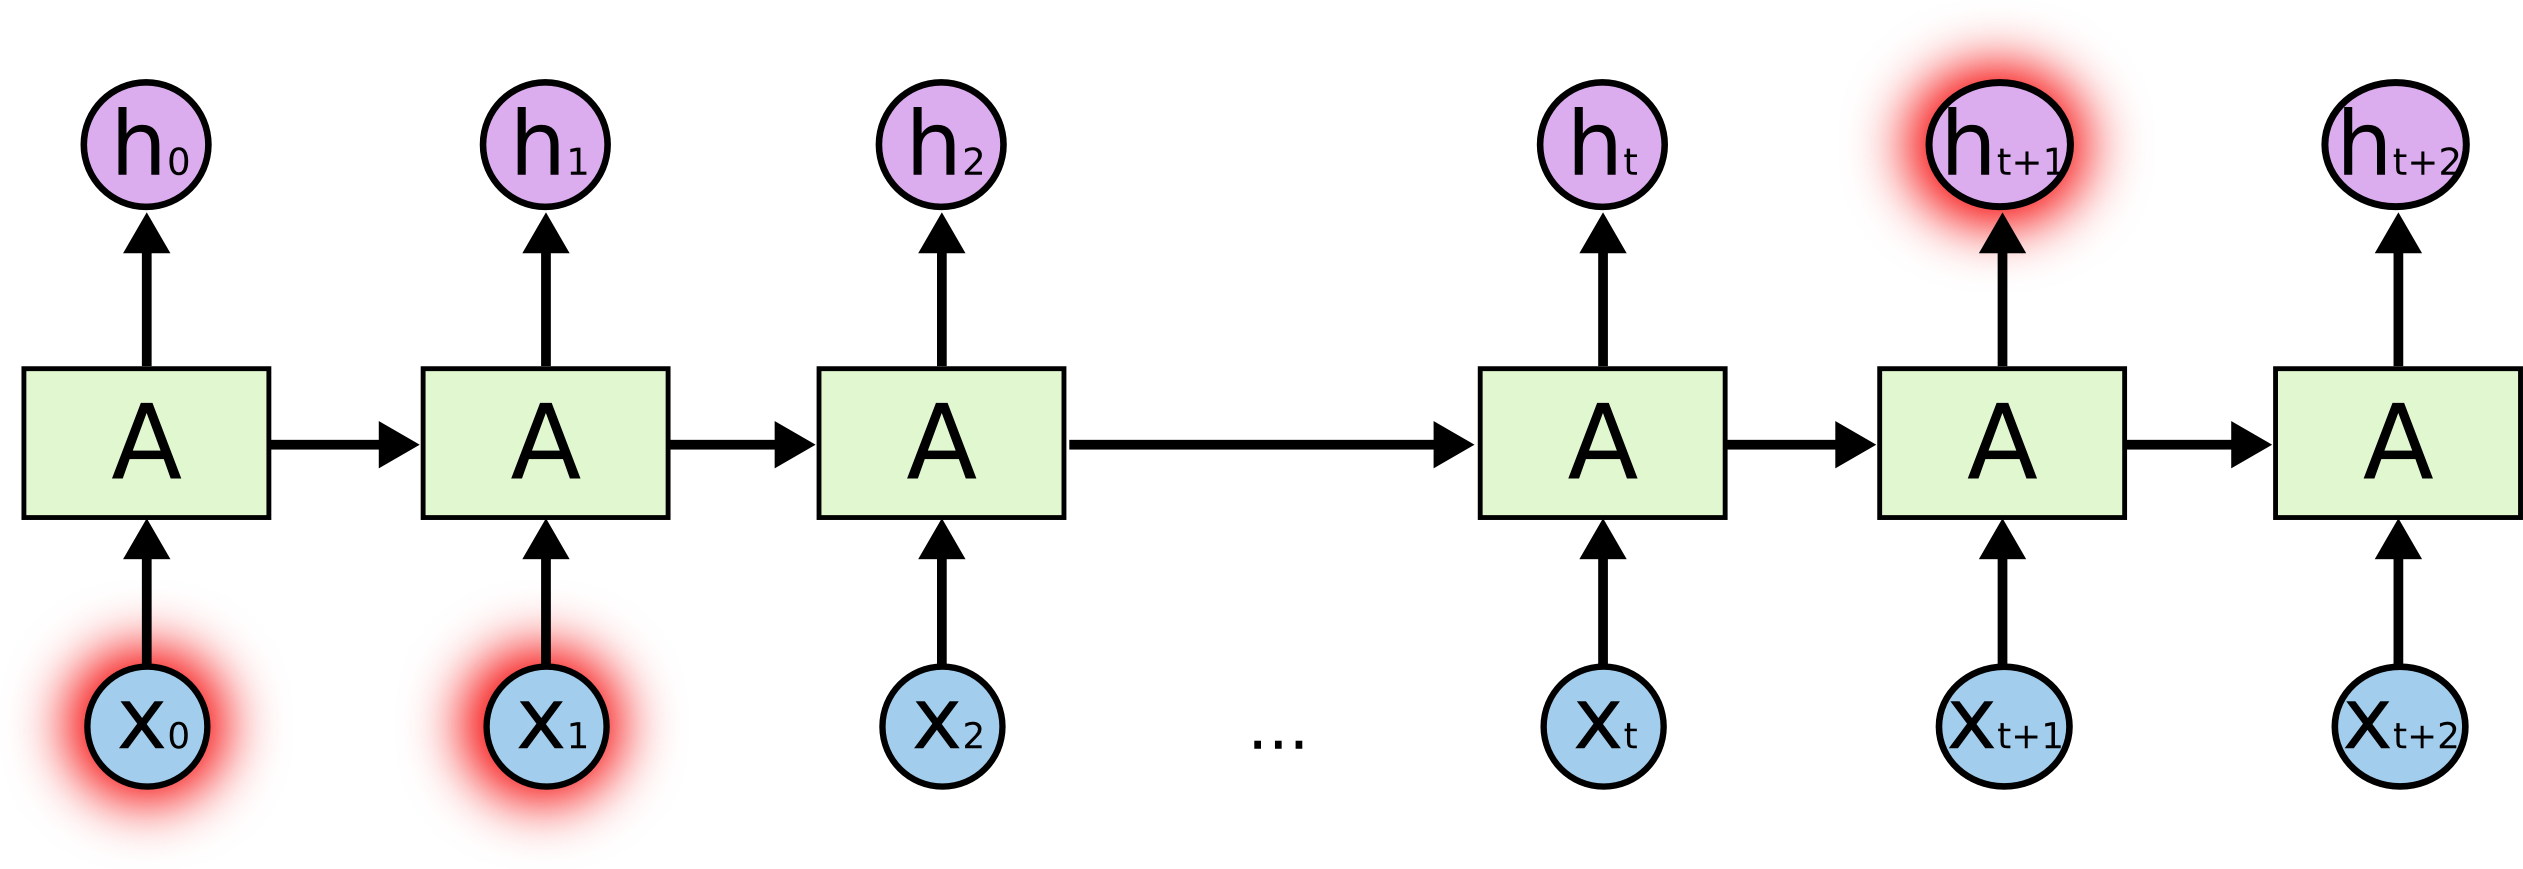
\includegraphics[width=0.8\textwidth]{fig/rnn.png}
\caption{RNN sequencing example (displays sequential input handling and state updating)~\parencite{olah_2015}}
\label{fig:rnn}
\end{figure}

Many problems hindered this approach, including a lack of concrete connection between distant words of a sequence. Additionally, as only a single hidden state was stored after each token was added, the weight (or visibility) of the beginning of the input could often become hidden and difficult for the model to recover~\parencite{hochreiter1997long}. 

For example, if a model is being trained to translate from English to Spanish, it can be reasonably assumed that the initial words of the English input have a strong correlation to the correct beginning tokens of the Spanish output. However, the model only contains the final latent state of the input, making it difficult to correctly decipher the beginning of the Spanish translation. Transformers were created to offer an alternative to this process, and they rely on a concept called attention and involve two components, an encoder and a decoder~\parencite{transformers:}. As \acrshort{bert} relies exclusively on encoders, they will be discussed.

\subsubsection{Encoders}
An encoder consists of two sub-layers, a self-attention layer that calculates the relation of each token to other tokens in the same input and a traditional feed-forward network. Self-attention is the concept of helping the model comprehend the relationships of words to other tokens in the input. For example, consider the sequence: \\

\textbf{The money has gone missing. Where is it?} \\

For a human, it would be easy to understand that \textbf{it} is referring to the \textbf{money}. But for a machine, it can be much more difficult to gather these types of contextual clues, especially if the corresponding words are separated~\parencite{hochreiter1997long}. Thus, self-attention generates “scores” for each input token with every other token which helps it understand the hidden/distant relationships. \\

The encoder takes the raw embedding sequence as input which is passed to the self-attention layer. The embeddings are slightly modified before being fed to the model, however. It is important for the computer to have some sense of the spatial relationships between words (the relative distances) to help with the positional aspect of the sequence. Thus, the model utilizes learned positional embeddings, which are the same size as the word embeddings themselves~\parencite{devlin2019bert:}. These positional vectors are added to the token vectors to create the real input:

\begin{figure}[h]
\centering
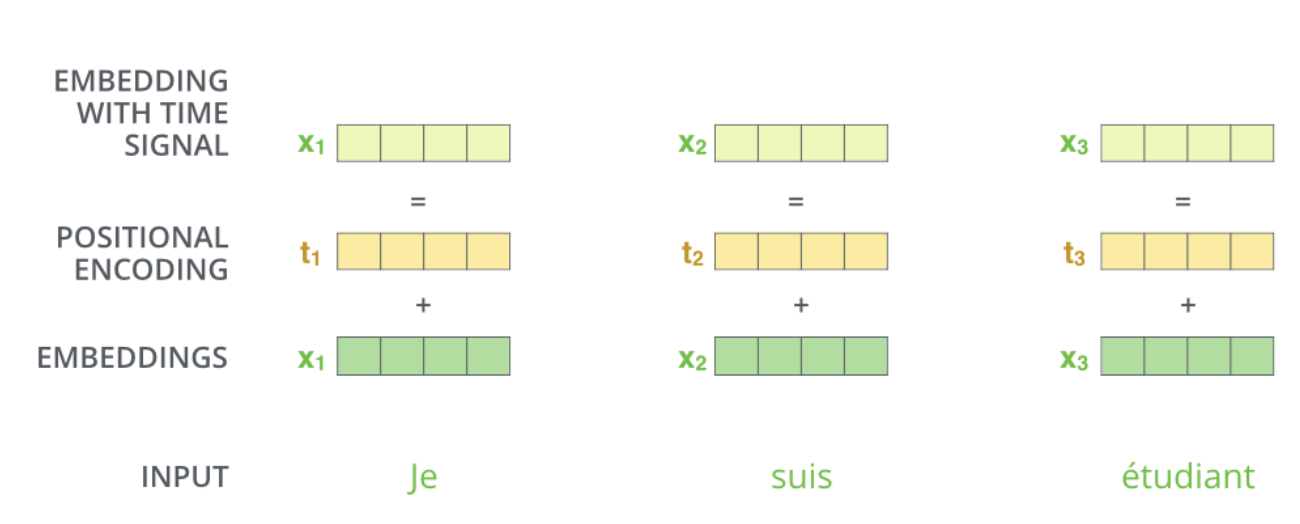
\includegraphics[width=0.8\textwidth]{fig/positional_encodings.png}
\caption{The basic addition of positional encodings to the input vectors before being fed to the model~\parencite{alammar_2018}.
}
\label{fig:positional_encodings}
\end{figure}

This layer then utilizes three matrices to generate a key, value, and query for each input token. For \acrshort{bert}, the embedding vectors are of length $768$, and each of these matrices has dimensions $768 \times 64$. For each token, the embedding vector is multiplied by the three matrices to get the key, query, and value vectors which each have a length of $64$. Then, the dot-product between the query vector and each token’s key is calculated to generate a score.

\begin{figure}[h]
\centering
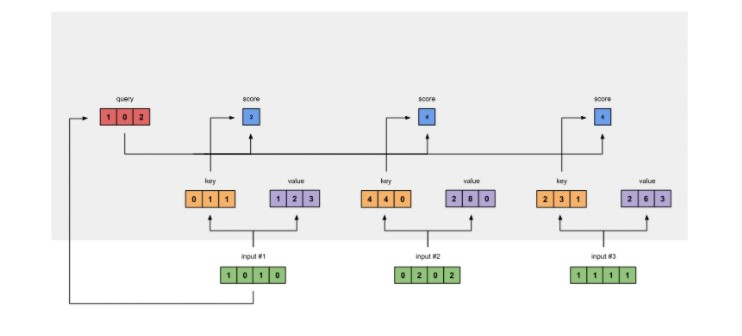
\includegraphics[width=0.8\textwidth]{fig/first_encoder_step.jpg}
\caption{Initial score generation for first token by taking a dot-product between the query vector and the key vectors for each token~\parencite{karim_2019}.)
}
\label{fig:first_encoder_step}
\end{figure}

The scores are then normalized with a $softmax$ function, defined by:
\begin{equation}
\label{eq:softmax}
S(y_i) = \frac{e^{y_i}}{\sum_{j\in y}e^{y_j}}, 
\end{equation}

\Cref{eq:softmax} takes a list of numbers and normalizes them into a probability distribution based on the exponential values of the inputs~\parencite{bengio_goodfellow_courville_2017}. These normalized scores are multiplied with the corresponding value vectors, which then are summed element-wise to get a final score for the token:

\begin{figure}[H]
\centering
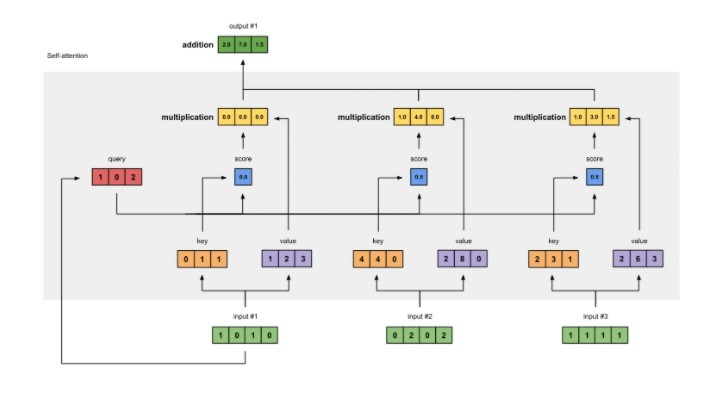
\includegraphics[width=0.8\textwidth]{fig/second_encoder_step.jpg}
\caption{The SoftMax function is applied to the initial score, then multiplied with the value vectors. The results are then summed to generate a final output for the first token~\parencite{karim_2019}.
}
\label{fig:second_encoder_step}
\end{figure}

This process is performed for each input token and is vectorized for faster computation. Transformers are able to utilize this process multiple times per encoder to generate what is known as multi-headed attention. In the case of \acrshort{bert}, this process is done $8$ separate times, each with a different key, query, and value matrix to get $8$ vectors of length $64$ for each input token. This makes the attention layer even more powerful and allows for more concrete connections to be encoded between words~\parencite{transformers:}. However, the feed-forward layer is not expecting each token to have multiple associated vectors, thus these outputs must be combined first before sending. To alleviate this problem, the vectors are all concatenated together to create a vector of length 512 $(8 \times 64)$, then multiplied with another parameter matrix of dimensions $512 \times 768$, to return to the original embedding size of $768$~\parencite{devlin2019bert:}, which is outlined here:

\begin{figure}[H]
\centering
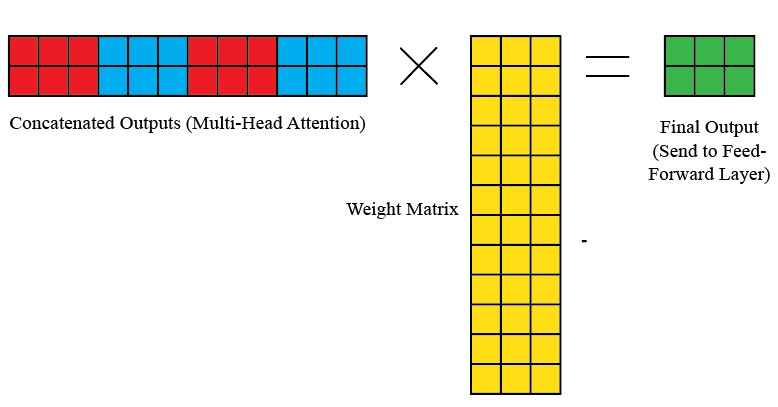
\includegraphics[width=0.8\textwidth]{fig/multi-head.jpg}
\caption{The outputs are concatenated as above then multiplied with the weighted matrix that is updated throughout training to get a final output with a 768 long vector for each token.
}
\label{fig:multi_head_attention}
\end{figure}

The overall attention process can be summarized as the following:
\begin{equation}
\label{eq:attention}
Attention\left(Q, K, V\right) = softmax\left(\frac{QK^\top}{\sqrt{d_k}}\right)V, 
\end{equation}

\Cref{eq:attention} outlines the attention function for a $(Q,K,V)$ value tuple. The results of the query and key product are divided by the square root of the size of the vectors (8 for~\acrshort{bert}) to normalize the outputs before applying softmax~\parencite{transformers:}.

This attention layer output is then passed to the fully-connected feed-forward neural network, which takes inputs of length 768 and returns an output of identical size based on a non-linear activation function as such:

\begin{figure}[H]
\centering
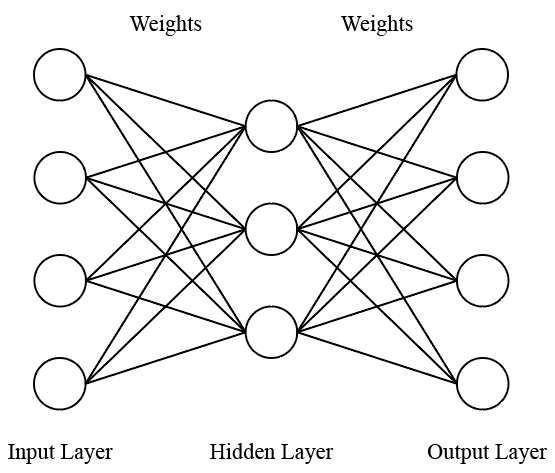
\includegraphics[width=0.8\textwidth]{fig/full_neural.png}
\caption{A sample fully-connected feed forward network with a hidden layer}
\label{fig:neural-network}
\end{figure}

The workings of a neural network have been extensively documented throughout machine learning literature, thus they will not be discussed in detail. However, the basic premise is very similar to the workings of \acrshort{rfs}, where a dot-product is calculated with learned weights, and then passed through an activation function, such as $\sigma$~\parencite{lecun2015deep}.

\subsubsection{General Working}
\acrshort{bert} employs 12 of these encoders, with both self-attention and feed-forward components, stacked on top of each other. Because the model is being used for classification, another final neural network is placed on top that takes the outputs of the encoders and generates a single probability for the entry~\parencite{sun2019finetune}.